\documentclass[
  bibliography=totoc,
  captions=tableheading,
  titlepage=firstiscover,
  twocolumn,
  %10pt,
]{scrartcl}

\setlength{\oddsidemargin}{0.0 cm}
\setlength{\evensidemargin}{0.0 cm}
\setlength{\topmargin}{-1cm}
\setlength{\textheight}{24 cm}
\setlength{\textwidth}{16 cm}

\pagestyle{plain}

\usepackage{fixltx2e}
\usepackage[aux]{rerunfilecheck}
\usepackage{polyglossia}
%\frenchspacing
\setmainlanguage[variant=british]{english}
\usepackage[intlimits]{amsmath}
\usepackage{amssymb}
\usepackage{mathtools}
\usepackage{fontspec}
\setsansfont{Helvetica}
\setmainfont{Charis SIL}
\setmonofont[Scale=0.92]{Source Code Pro}
\defaultfontfeatures{Ligatures=TeX}
\usepackage[
  math-style=ISO,
  bold-style=ISO,
  sans-style=italic,
  nabla=upright,
  partial=upright,
]{unicode-math}
\setmathfont{Tex Gyre Pagella Math}
%\setmathfont{Asana Math}
%\setmathfont{Latin Modern Math}
\setmathfont[range={\mathscr, \mathbfscr}]{XITS Math}
\setmathfont[range=\coloneq]{XITS Math}
\setmathfont[range=\propto]{XITS Math}
\removenolimits{\int}
\let\hbar\relax
\DeclareMathSymbol{\hbar}{\mathord}{AMSb}{"7E}
\DeclareMathSymbol{ℏ}{\mathord}{AMSb}{"7E}
\usepackage[autostyle]{csquotes}
\usepackage[
  locale=US,
  separate-uncertainty=true,
  per-mode=symbol-or-fraction,
]{siunitx}
\usepackage[version=3]{mhchem}
\usepackage{xfrac}
%\usepackage[section, below]{placeins}
\usepackage[
  labelfont=bf,
  font=small,
  width=0.9\textwidth,
]{caption}
\usepackage{subcaption}
\usepackage{graphicx}
\usepackage{grffile}
\usepackage{float}
\usepackage[italic]{hepnicenames}
\floatplacement{figure}{htbp}
\floatplacement{table}{htbp}
\usepackage{booktabs}
\usepackage{pdflscape}
\usepackage[
  sorting=none,
]{biblatex}
\addbibresource{main.bib}
\usepackage{microtype}
\usepackage{blindtext}
\usepackage[
  unicode,
  pdfusetitle,
  pdfcreator={},
  pdfproducer={},
]{hyperref}
\usepackage{bookmark}
\usepackage[shortcuts]{extdash}
\usepackage{tikz}
\captionsetup{width=0.45\textwidth}


\captionsetup{width=0.45\textwidth}

\begin{document}

\twocolumn[{%
\begin{center}
  {\LARGE \textbf{\textsf{Top Quark Seminar 11}}} \\
  \vspace{1em}
  {\Large \textbf{\textsf{Igor Babuschkin}}} \\
  \vspace{1em}
  {\large \textbf{\textsf{6th January 2015}}}
  \section*{Summary of \enquote{Top quark precision physics at the International Linear Collider}}
\end{center}
}]

The article\cite{ilc} is a white paper detailing in how far an International Linear Collider (ILC) could provide opportunities for performing precision measurements of the top quark.
The ILC—should it be constructed—will be a linear electron-positron collider with possible center-of-mass energies exceeding that of two top quarks.
The process considered by the authors is $e^+e^-\to t\overline{t}$.
They estimate that the ILC will be able to collect $10^6$ $e^+e^-\to t\overline{t}$ events (at an integrated luminosity of $\SI{500}{fb}^{-1}$) with little background.

The ILC would be the first experiment to allow the study of top quarks using a precisely defined leptonic initial state, meaning that energy and polarization of the initial electron-positron system could be set precisely.
One caveat to this is that the electron and positron can radiate photons, in which case the energy available to the studied process is actually smaller.
The resulting energy distribution is referred to as the \emph{luminosity spectrum}.

While summarizing experimental studies, the authors also investigate in how far current theoretical calculations are sufficiently developed to be useful in interpreting the new ILC results.

As an example of an important measurement that could be performed at the ILC, the authors present the measurement of the shape of the $t\overline{t}$ cross section close to $\sqrt{s} = 2 m_t$.
Different predictions for the cross section shape from theory can be seen in figure \ref{crosssection}.
Fitting the cross section shape can yield precise values for the top quark mass, the strong coupling $\alpha_s$ and other observables.

\begin{figure}
  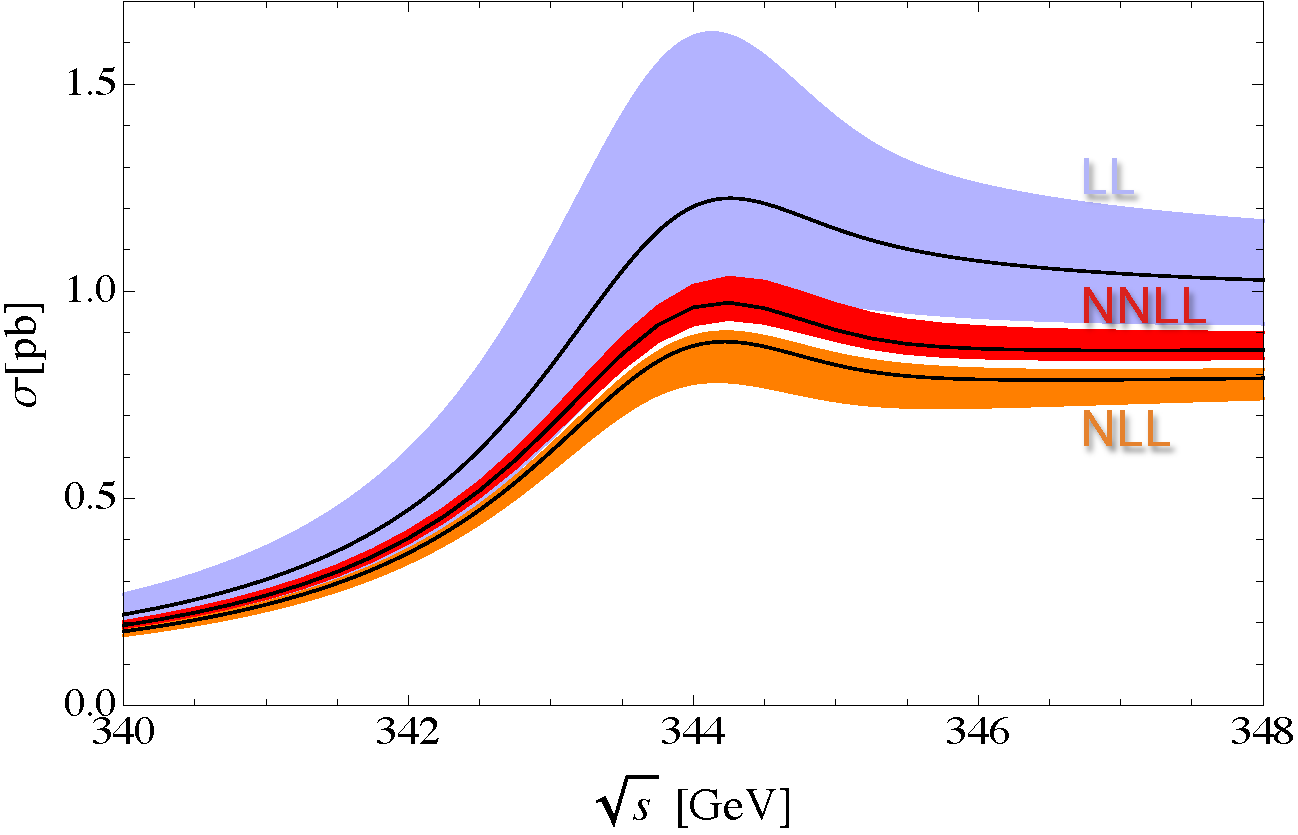
\includegraphics[width=0.45\textwidth]{./figures/TotCrossCombined.pdf}
  \caption{Shape of the $e^+e^-\to t\overline{t}$ cross section according to several theoretical calculations with improving precision.\cite{ilc}}
  \label{crosssection}
\end{figure}

Another interesting measurement is the precise determination of the interaction of the top quark with $γ$ and $Z^0$.
The interaction vertex can be parameterized in terms of form factors.
By controlling the initial state polarization, individual form factors could be isolated and measured with high precision.
This type of measurement, which has already been performed at LEP for other final states, could now be extended to top quarks.
The authors cite a paper\cite{study} in which sensitivity studies for the individual form factors have been performed and which shows that the precision achievable at the ILC clearly surpasses that of the LHC.
It is argued that the higher precision of the ILC could make New Physics effects appearant in the coupling of the top to photon and $Z^0$ boson.
A few proposed models are presented.
The authors conclude that while the ILC could offer a glimpse at New Physics, detector performance and event reconstruction have to be excellent.
They also emphasize that theoretical predictions have to be improved to make use of the new experimental results.

\nocite{*}
\printbibliography

\end{document}
